\subsection{Experimentacion sobre Simmulated Annealing}

Al momento de experimentar sobre Annealing, debemos tener en cuenta que cosas contribuyen a la calidad de la solución final. Es sobre los siguientes puntos que hacemos foco a la hora de experimentar:

\begin{description}
\item[El “plano” de soluciones:] Dado que nos encontramos frente a una función con dominio multidimensional, se vuelve inviable representar gráficamente la función. Sin embargo basta con tomar un caso simplificado como el de la figura \ref{fig:minimo-local} para poder ver que la forma del plano puede no prestarse a una exploración exitosa desde algunos puntos. Este caso es bastante difícil de recrear manualmente dado que estamos lidiando con una función multidimensional con un dominio no ordenado, por este motivo va a ser obviado en nuestra experimentación práctica.

\item[La solución inicial:] Esta misma tiene un gran impacto sobre el desempeño del algoritmo por diversos motivos, ya que la temperatura inicial y final son calculadas a partir de la misma, así como también el punto de partida a la hora de explorar el vecindario. 

\item[La cantidad de resets:] Los resets o ciclos de temperatura existen como un método de backtracking a la hora de llegar a un camino sin salida, es decir, explorar todo un vecindario sin encontrar una solución mejor a la actual.

\item[El azar:] Como se mencionó antes, la probabilidad de aceptar una solución termina siendo definida por un número uniformemente aleatorio, por lo que al correr repetidas veces el programa podemos llegar a resultados muy distintos.

\item[La cantidad de exploraciones:] El factor $\alpha$ dentro de la ecuación de enfriamiento depende de la cantidad de iteraciones aproximadas para que la temperatura actual sea la misma que la final. Si bien este número no es más que una guía (puesto que el algoritmo puede seguir buscando soluciones a medida que encuentre mejores) afecta la curva de temperatura directamente. 

\end{description}


Dado que la solución presentada por Annealing no es determinista, decidimos tomar el siguiente enfoque a la hora de realizar nuestros experimentos.
Hacemos 10 corridas de Simulated Annealing sobre el mismo dataset y solución inicial, tomando el promedio de energía y temperatura de las soluciones propuestas por el algoritmo.

\subsubsection{Cantidad de exploraciones}
Si bien es difícil cuantificar el impacto de un cambio de parámetro sobre Annealing (dado que la duración del algoritmo puede variar al azar y según el plano de soluciones), proponemos que se puede observar la saturación de cantidad de iteraciones esperadas para el enfriamiento. Es decir, variando el parámetro $\alpha$ -la cantidad de iteraciones esperadas para que la temperatura actual iguale a la final- podemos sugestionar a la función de enfriamiento, para que incrementa en mayor o menor medida la temperatura.

Esto termina provocando que el algoritmo ejecute más o menos iteraciones sobre la solución.
Proponemos que incrementar desmedidamente este valor para lograr mayor exploraciones, no necesariamente recompensa el costo de tiempo asociado con la mejor solución potencial. 

Para realizar
\begin{figure}[H]
	\centering
	\begin{minipage}[t]{.30\textwidth}
		\centering
		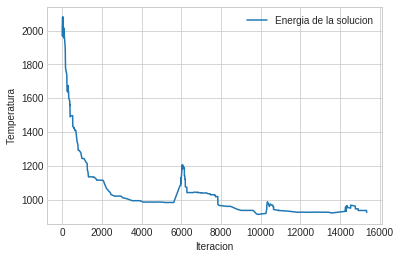
\includegraphics[scale=0.4]{annealing/1000-it-energia}
		\caption{1.000 iteraciones}
	\end{minipage}\qquad
	\centering
	\begin{minipage}[t]{.30\textwidth}
		\centering
		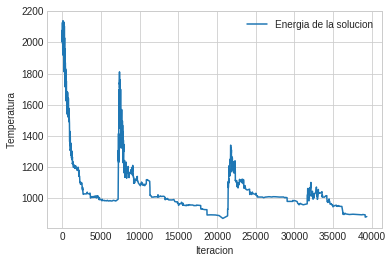
\includegraphics[scale=0.4]{annealing/10000-it-energia}
		\caption{10.000 iteraciones}
	\end{minipage}\qquad
	\centering
	\begin{minipage}[t]{.30\textwidth}
		\centering
		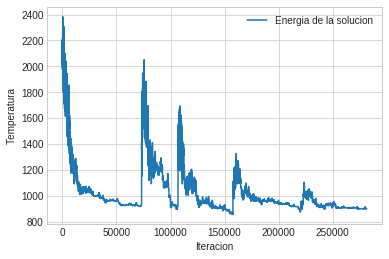
\includegraphics[scale=0.4]{annealing/100000-it-energia}
		\caption{100.000 iteraciones}
	\end{minipage}\qquad
	\centering
	\begin{minipage}[t]{.30\textwidth}
		\centering
		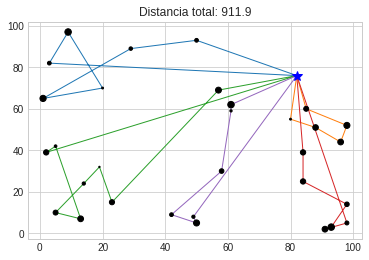
\includegraphics[scale=0.4]{annealing/1000-it-grafo}
	\end{minipage}\qquad
	\centering
	\begin{minipage}[t]{.30\textwidth}
		\centering
		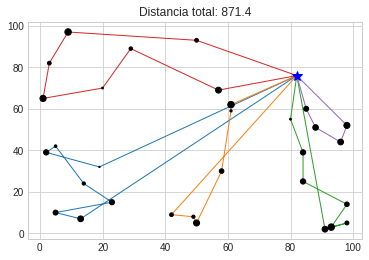
\includegraphics[scale=0.4]{annealing/10000-it-grafo}
	\end{minipage}\qquad
	\centering
	\begin{minipage}[t]{.30\textwidth}
		\centering
		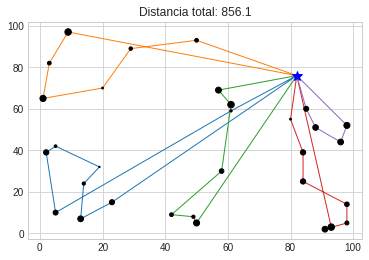
\includegraphics[scale=0.4]{annealing/100000-it-grafo}
	\end{minipage}\qquad
\end{figure}	

Como podemos ver, usando un parámetro chico como $\alpha$ = 1.000, obtenemos una distancia total (en promedio) de 912. Como podemos ver, esto decrementa rápidamente la temperatura, lo cual no nos permite aprovechar al máximo la capacidad de annealing de aceptar soluciones malas, haciendo que el algoritmo caiga fácilmente en óptimos locales.
\vskip 1em

Al utilizar un valor más grande ($\alpha$ = 10.000) vemos cómo se producen fluctuaciones de energía más grandes, y las temperaturas de reiniciado tambien son mas altas. En cuanto a la distancia total final, obtenemos 871.4, un 5\% de mejora respecto a la corrida anterior. Y en cuanto a la cantidad final de iteraciones del algoritmo, observamos que se trata de un poco menos que el triple.
\vskip 1em

Para el parámetro saturado, es decir ($\alpha$ = 100.000) podemos ver cómo se producen fluctuaciones de temperatura todavía más grandes, y se logra una mejora por sobre el caso anterior. Sin embargo está vez solo se trata de un 1.75\%, tomando 7 veces más iteraciones para terminar de explorar.
\vskip 1em

Visto esto, concluimos que efectivamente se puede llegar a un punto de saturación a la hora de elegir el alpha, lo cual incurre en un costo de tiempo de cálculo. En vistas de esto a la hora de tratar de obtener la mejor solución posible, antes que tratar de maximizar la cantidad de soluciones exploradas por una corrida del algoritmo, es recomendable correr múltiples veces el mismo con un $\alpha$ menor. Dado que al depender de un valor al azar para aceptar una solución, podemos llegar a obtener mejores caminos de esta forma.

